Accurate modeling of a wide variety of functions enables the imputation of missing values in time series data and the creation of continuous data for further processing. We assume that for a given set of observations, there exists an underlying function that describes the data. Our goal is to model this underlying function such that we can predict all function values and therefore impute missing values. Empirical real-world data often consist of discrete measurements that need to be imputed to apply continuous mathematical tools.

One example from the field of astronomy works on luminosity values from Cepheid variable stars. Cepheid stars change their luminosity periodically, as visible in \autoref{fig:cepheid_image}. Crucially, as discovered by the astronomer Henrietta Leavitt, the frequency of those periods directly correlates to their absolute luminosity. Knowing the absolute luminosity of a star is very useful, as it allows astronomers to calculate the distance to that star.

Before the twentieth century it was not possible to measure distances of more than a few hundred lightyears. This was important for the debate of whether the Andromeda galaxy, formerly known as the Andromeda nebula, is part of our own galaxy or rather a galaxy of its own. By discovering cepheid variable stars in the Andromeda galaxy and using Leavitts Law, the distance could be calculated and the Andromeda galaxy was recognized as such. \cite{gaßnerAstroBook}

\begin{figure}[h]
	\centering
	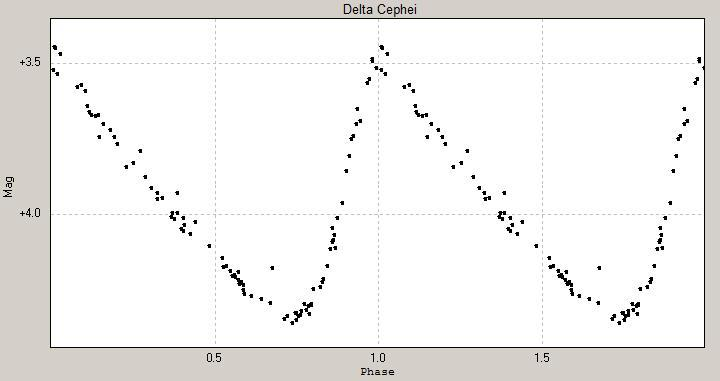
\includegraphics[width = 0.5\textwidth]{figures/Cephei}
	\caption{Lightcurve data from the variable star Delta Cephei, over two periods. \tiny\url{ https://de.wikipedia.org/wiki/Datei:Delta_Cephei_lightcurve.jpg}}
	\label{fig:cepheid_image}
\end{figure}

Estimating the underlying function given the provided data in \autoref{fig:cepheid_image} would allow removal of the present noise and apply further processing, such as calculating the extrema of that function and computing the frequency based on that. This would then enable us to calculate the distance to the star from which the data have been collected.

We use synthetic time-series data to train a model that interpolates the underlying function and imputes missing values. We sample our data from a multivariate normal distribution and train a transformer model to estimate unseen values given a certain number of context points. We follow the general approach from \citet{seifner2025zeroshotimputationfoundationinference}, while using transformers instead of LSTMs and estimating the actual function, instead of derivatives. We compare our results with a Gaussian Process baseline and discuss how the prior distribution and number of context points influence the performance. Finally, we use our transformer model to impute missing values for Cepheid star luminosity values and show that the model trained on synthetic data is applicable to real world data.

The entire code base, models, and datasets are available online on github\footnote{\url{https://github.com/ChristianSchultze/in-context-function-estimation.git}} and sciebo\footnote{\url{https://uni-bonn.sciebo.de/s/oMqWpRRyPM6obzZ}}.
The source code is pip installable, core scripts can be configured through command line arguments. The model configuration for training and evaluation, as well as hyper parameters, is configured by a yml config file. The sampling code for synthetic data is covered by automatic tests and the entire code is linted and checked by a static type checker for python.